\documentclass[10 pt,usenames,dvipsnames, oneside]{article}
\usepackage{../../../modelo-ensino-medio}



\begin{document}

\begin{center}
  \begin{minipage}[l]{3cm}

\includegraphics[width=2cm]{logo}    
\end{minipage}\hfill
\begin{minipage}[r]{.8\textwidth}
 {\Large \scshape Atividade: Retornando ao Estádio Mineirão}  
\end{minipage}
\end{center}
\vspace{.2cm}

\ifdefined\prof
%Habilidades da BNCC
% \begin{objetivos}
% \item 
% \end{objetivos}

%Caixa do Para o Professor
\begin{goals}
%Objetivos específicos
\begin{enumerate}
\item Trabalhar a intercessão entre os  conjuntos solução de uma equação da elipse e uma equação linear
\end{enumerate}

\tcblower

%Orientações e sugestões
\begin{itemize}
\item No item \titem{a)}, é interessante que o aluno esboce a figura, de forma a verificar possíveis interseções. Auxilie-o a perceber que os pontos de interseção entre a reta e as elipses são pontos que pertencem tanto á reta quanto a cada elipse, sendo portanto soluções que satisfazem aos pares respectivos de reta e elipse. Além disso, o aluno precisará considerar ainda uma direção estabelecida, que implica na busca das interseções que estejam no segundo quadrante.
\item No item  \titem{b)}, a situação é análoga à de \titem{a}), mas em lugar de termos a reta que modela o chute, temos a direção estabelecida por dois pontos: o centro e o ponto $(1,1)$. Caberá ao aluno determinar qual seria a equação dessa reta, o que pode ser feito considerando seus conhecimentos sobre funções afins, e a seguir, atuar conforme feito no item \titem{a)}.
\end{itemize}
\end{goals}

\bigskip
\begin{center}
{\large \scshape Atividade}
\end{center}
\fi

Manoel Rezende de Mattos Cabral, mais conhecido como Nelinho, foi um jogador de futebol brasileiro que atuava como lateral direito e participou como titular da seleção brasileira nas copas de 1974 e 1978. Em 1979, ao ser desafiado por uma emissora de televisão, Nelinho conseguiu chutar uma bola para fora do estádio do Mineirão, estando dentro do campo (veja a façanha de Nelinho em \url{https://www.youtube.com/watch?v=psJJEdZHpcU}).


Na Atividade \hyperref[estadio]{Estádio de Futebol} da seção anterior, consideramos que o Estádio do Mineirão pode ter o seu contorno externo representado por uma elipse de equação $9x^2 = 144 - 16y^2$, em um sistema de coordenadas cartesianas, conforme indicado na figura a seguir, com o centro do campo coincidindo com a origem $(0,0)$ e de forma que as unidades de medida reais estejam em escala com este sistema.

\begin{figure}[H]
\centering

\noindent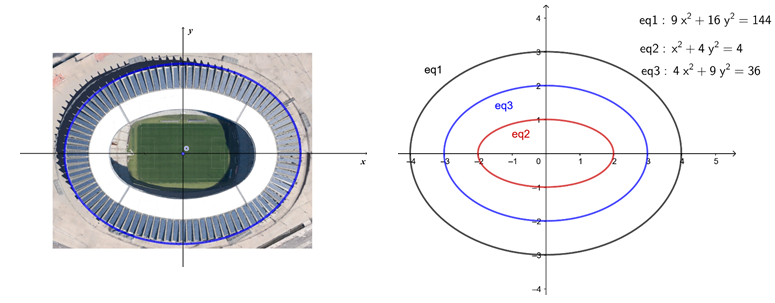
\includegraphics[width=400bp]{estadio2.png}
\end{figure}
\begin{enumerate} 

\item{}
Assumindo uma vista aérea conforme representada nas figuras anteriores, suponha que Nelinho tenha chutado a bola a partir do centro do campo em direção ao corner do time adversário (2\super{o} quadrante) em trajetória retilínea (numa vista aérea) que segue a equação $y = -x$. Em que pontos do plano cartesiano a projeção da trajetória dessa bola cruzará as três elipses?

\item{}
Novamente, Nelinho está no centro do campo de jogo e deu um outro chute, agora na direção do ponto $(1,1)$, de forma que, numa vista aérea, a bola segue uma trajetória retilínea e sai do estádio. Em que pontos (no primeiro quadrante) a vista aérea desse chute intersecta as três elipses?

\end{enumerate}

\ifdefined\prof
\begin{solucao}

\begin{enumerate}
\item $\displaystyle eq_1:(-\frac{12}{5},\frac{12}{5} );\ \newline eq_2:(-\frac{2\sqrt{5}}{5},\frac{2\sqrt{5}}{5});\  \newline eq_3:(-\frac{6\sqrt{13}}{13},\frac{6\sqrt{13}}{13})$
\item $\displaystyle eq_1:(\frac{12}{5},\frac{12}{5} );\ \newline eq_2:(\frac{2\sqrt{5}}{5},\frac{2\sqrt{5}}{5});\  \newline eq_3:(\frac{6\sqrt{13}}{13},\frac{6\sqrt{13}}{13})$
\end{enumerate}

\end{solucao}
\fi

\end{document}